% sec_a.tex: Introduction, Problem definition, Motivation, Related work

\section{Introduction}\label{sec:intro}
A database that crashes gets fixed the same day. A database that returns one wrong row can go unnoticed for years: the oldest bug CODDTest found had sat in MySQL for 14 years~\cite{coddtest}. These are \emph{logic bugs}. The system accepts a valid statement, reports success, and returns a wrong result or stores a wrong state, so the application has nothing to catch.

Finding them is hard because of the oracle problem. To see that an answer is wrong you need the right one, and writing a second SQL engine to compute it is out of reach. The four papers we review share a cheaper trick: ask the same system the same question in two ways that must agree. Figure~\ref{fig:oracles} shows one real bug per paper. CODDTest~\cite{coddtest} replaces an expression by its precomputed value. DDLCheck~\cite{ddlcheck} rebuilds a schema without its history. Radar~\cite{radar} drops optional metadata such as indexes. WriteCheck~\cite{writecheck} replays concurrent transactions one after another.

We ask how the equivalence each oracle relies on decides which bugs it can find, and how well each paper's experiments back its claims. The report contributes three things:
\begin{itemize}[leftmargin=1.1em,itemsep=1pt,topsep=2pt]
\item \textbf{One model for four oracles} (Section~\ref{sec:problem}, Figure~\ref{fig:model}).
\item \textbf{A coverage map} of the failures each oracle can observe (Table~\ref{tab:coverage}): each is strongest somewhere else, and all four share one blind spot.
\item \textbf{An evidence audit} (Sections~\ref{sec:experiments} and~\ref{sec:discussion}): verdicts per claim, and two reporting patterns that block any ranking by bug count.
\end{itemize}
All measurements come from the four papers; the model, matrices and verdicts are ours. NoREC and TLP~\cite{norec,tlp}, two earlier oracles, serve as background.

\section{Problem definition and discussion}\label{sec:problem}
\subsection{High-level description}
Picture a shop database with a \texttt{Product} table holding stock and reserved units. Whatever its past, some pairs of executions must agree. Replacing \texttt{quantity - reserved} by its value cannot change which products a query lists. A table created in its final form must behave like one that got there through three migrations. A query that never names an index must return the same rows with or without it. Two committed transactions must leave a state that some serial order could also produce. Logic-bug testing searches for inputs that break one of these promises.

\subsection{Formal definition and search objective}\label{sec:formal}
Let $E$ be a DBMS. A database state is $D=(S,V,M,H)$: visible schema $S$, stored values $V$, optional metadata $M$ such as indexes and constraints, and construction history $H$ with whatever hidden state it left. A workload $W$ is a query, a statement sequence or a set of transactions, and $C$ is the context (dialect, session settings, isolation level). The observation $O(E,D,W,C)$ is what the oracle compares: result rows, statement success, final contents or the schema. A transformation $T$ maps $(D,W)$ to $(D',W')$, and a precondition $P$ says when both pairs ask the same question.

\begin{tcolorbox}[enhanced,colback=panelbg,colframe=panelborder,boxrule=0.5pt,arc=3pt,left=7pt,right=7pt,top=4pt,bottom=4pt]
\small
\textbf{Given} $E$, $C$, a space of pairs $(D,W)$, a transformation $T(D,W)=(D',W')$ and a precondition $P$.
\textbf{Find} triples $(D,W,T)$ for which
\[
P(D,W,C)\;\wedge\;O(E,D,W,C)\not\equiv O(E,D',W',C),
\]
each reported with a reduced test case that reproduces it.
\end{tcolorbox}

Such a triple is a \emph{candidate}. It becomes a defect only after $P$ is confirmed, permitted nondeterminism is ruled out and the documentation is checked. The four papers do not use this notation; it is our common frame.

\subsection{Detailed discussion of the definition}\label{sec:detailed}
Each paper is one choice of $T$, $P$ and $O$, and Figure~\ref{fig:model} shows where each one intervenes. CODDTest and WriteCheck change the workload, DDLCheck the history, Radar the metadata. The precondition is what keeps each comparison honest. CODDTest needs a deterministic expression and a state that does not move between the auxiliary and the folded query. DDLCheck needs the rebuilt schema to match in every property later statements can see. Radar needs a read-only query that does not depend on what was dropped. WriteCheck needs writes that never use values read earlier in their transaction.

\begin{figure}[!tb]
\centering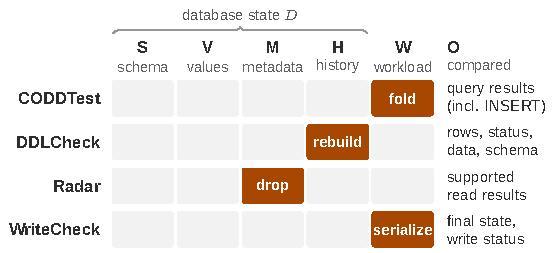
\includegraphics[width=\columnwidth]{fig_model}
\caption{\textbf{Where each oracle intervenes.} Orange marks the part of the state $D$ or the workload $W$ that the transformation changes; grey parts stay identical. The right column is the observation $O$ the oracle compares.}
\label{fig:model}
\end{figure}

\paragraph{What ``$\equiv$'' means.} Unordered results compare as multisets: order is ignored, duplicate counts are not, since a set would hide a dropped or duplicated row. NULLs, types, collation, rounding and errors need the same treatment on both sides, which is why CODDTest avoids extreme floating-point values and adds explicit casts in SQLite~\cite[Sec.~4.1]{coddtest}. For data-changing workloads, equal query output is not enough, because two INSERTs can both succeed and store different values. That is why DDLCheck and WriteCheck compare final state, and DDLCheck the schema too.

\subsection{Pseudoalgorithm}
Algorithm~\ref{alg:oracle} is the loop the four methods share. The real tools add steps: CODDTest runs an auxiliary query before folding, and WriteCheck must run the concurrent schedule before it knows which serial order to replay. Reduction (line~10) is the most underestimated step. Radar's authors spent three weeks reducing 1,663 raw reports to 42 unique bugs~\cite[Sec.~4.2]{radar}, and every shrink must keep the mismatch alive, because a smaller query can take a different plan and lose the bug.

\begin{algorithm}[!tb]
\caption{Generic metamorphic logic-bug search}
\label{alg:oracle}
\small
\begin{algorithmic}[1]
\Require DBMS $E$, context $C$, generator $G$, oracle family $F$, budget
\While{budget remains}
  \State $(D,W)\gets G.\textit{NextCase}(C)$
  \State $(T,P)\gets F.\textit{Choose}(D,W,C)$
  \If{\textbf{not} $P(D,W,C)$} \textbf{continue} \EndIf
  \State $(D',W')\gets T(D,W)$
  \State $A\gets\textit{RunFromCleanState}(E,D,W,C)$
  \State $B\gets\textit{RunFromCleanState}(E,D',W',C)$
  \If{\textbf{not} \textit{Equivalent}$(A,B,F.\mathit{rules})$}
    \State $\mathit{case}\gets\textit{ReduceKeepingMismatch}(D,W,T,C)$
    \State \textit{Record}$(\mathit{case},\text{version},\text{seed})$
  \EndIf
\EndWhile
\end{algorithmic}
\end{algorithm}

\begin{takeaway}
An oracle is a triple $(T,P,O)$. Each paper's contribution is a new transformation, the precondition that makes it safe, and an observation rich enough to show the bug.
\end{takeaway}

\section{Motivation}\label{sec:motivation}
\subsection{Running example}
Back to the shop. Each paper suggests a different test against \texttt{Product}. \textbf{Expressions:} filter on available stock, then rerun with the subquery replaced by its value. \textbf{History:} add \texttt{reserved} through \texttt{ALTER TABLE} and compare with a table created with it. \textbf{Metadata:} run the stock report with and without an index on \texttt{quantity}. \textbf{Transactions:} let two checkouts update \texttt{reserved} at once, then compare with a serial replay. One passing test says little about the others: an expression test on a fresh table never sees what a migration leaves behind, and a single-connection test never sees a write conflict. The transaction test needs care too. A checkout that reads \texttt{quantity} and later writes a value computed from it is outside WriteCheck's scope, and a race there is an application bug.

\subsection{Why it matters and what makes it hard}
DBMS developers receive short, reproducible cases that point at a wrong assumption in optimizer or executor code; CODDTest reports 33 of its 45 bugs fixed by publication~\cite{coddtest}. Application teams benefit because a wrong stored state outlives the request that caused it. Four things make the problem hard:
\begin{enumerate}[leftmargin=1.3em,itemsep=0pt,topsep=2pt]
\item \emph{Valid SQL is not a valid test.} A comparison needs a rule for NULLs, types, errors and nondeterminism.
\item \emph{The reference is not independent.} Both runs use the system under test, so a fault on both paths cancels out.
\item \emph{State is invisible.} Schema changes and metadata leave internal state that no query shows.
\item \emph{Concurrency has many right answers.} Choosing the serial order to compare against is itself a model.
\end{enumerate}

\subsection{Limitations of existing work, and can it be extended?}
Each paper narrows its comparison to make $P$ checkable, and each narrowing leaves a gap. \textbf{CODDTest} works on a fixed state; 4 of the 14 bugs it missed in its SQLite comparison involved indexes~\cite[Sec.~4.2]{coddtest}. \textbf{DDLCheck} needs a schema description complete enough to rebuild from; a lost property makes the reference wrong. \textbf{Radar} covers read-only queries, since dropping a UNIQUE constraint legitimately changes whether an INSERT succeeds. \textbf{WriteCheck} covers neither read-dependent writes nor read anomalies, and its serial order assumes a conflict model that semi-consistent reads and missing gap locks violate.

Can the gaps be closed? Partly. CODDTest's folding and Radar's raw copy both take a given state, so both could run on states that DDLCheck's histories produce, and DDLCheck already checks which of its bugs Radar could catch~\cite[Table~4]{ddlcheck}. WriteCheck is harder to extend: once a write uses a value read earlier, a serial replay may legitimately read something else, and the reference is no longer defined. None of these extensions is demonstrated.

\section{Related work}\label{sec:related}
We group the papers by how they build the reference run, following the columns of Figure~\ref{fig:oracles}.

\paragraph{Query consistency: CODDTest and Radar.} Both keep the stored data and change how a read is answered. CODDTest borrows constant folding from compilers~\cite[Sec.~3]{coddtest}. An auxiliary query evaluates an expression or subquery, and its value replaces it in the original query; a row-dependent expression becomes a CASE map, because one constant would change the meaning. It extends SQLancer and was evaluated on five DBMSs. Radar builds a raw copy that keeps the data but drops indexes and constraints, then checks $E(D,Q)\equiv E(\mathrm{raw}(D),Q)$~\cite{radar}. It excludes queries that name an index, read a default value, or call identity or nondeterministic functions~\cite[Sec.~3.2.2]{radar}, and it steers generation toward metadata it has not tried. In the MySQL bug of Figure~\ref{fig:oracles}, an index on a \texttt{DOUBLE ZEROFILL} column makes a query return a row that the raw copy correctly omits.

\paragraph{Schema history: DDLCheck.} DDLCheck generates CREATE, ALTER and DROP sequences, reads the resulting schema back, and synthesizes a shorter sequence that creates it directly~\cite{ddlcheck}. The same later statements run on both. In MDEV-35122, MariaDB keeps a dropped BLOB as a hidden column, so a later INSERT fails with ``row size too large'' while the directly created table accepts it~\cite[Listing~1]{ddlcheck}. The revealing statement is an INSERT, which no query-only oracle compares.

\paragraph{Transactions: WriteCheck.} WriteCheck targets write-specific serializability (WSS): concurrent transactions must leave the state that some serial order would~\cite{writecheck}. A write may use explicit values or values it reads itself (\texttt{SET c = c + 1}) but not values from an earlier read. The serial order follows the order in which transactions finished, a pattern the authors call First Commit/Rollback First Scheduled (FCRFS), and the check is $\mathrm{State}(D_0,H_c)=\mathrm{State}(D_0,H_f)$. FCRFS models how a system resolves conflicts, so semi-consistent reads and missing gap locks can break it without any implementation bug~\cite[Sec.~6.4]{writecheck}. In TiDB\#42486 a transaction that should abort commits, and the table keeps a value the serial replay deletes.

\subsection{Comparison and earlier methods}\label{sec:compare}
Table~\ref{tab:coverage} turns the four mechanisms into a coverage map. Each oracle owns at least one row that no other covers, so they complement each other. Overlaps are partial: Radar's half mark on schema changes reflects DDLCheck's own finding that Radar can expose 13 of its 21 schema bugs through a later SELECT~\cite[Table~4]{ddlcheck}. The last row is empty for all four.

\begin{table}[!tb]
\caption{\textbf{What each oracle can observe.} \yes\ in scope; \half\ partly or indirectly; \no\ out of scope. Only failures exposed by the pairwise comparison count, not crash checks. Our reading of each paper's design and limitations.}
\label{tab:coverage}
\centering\footnotesize\setlength{\tabcolsep}{1.6pt}\renewcommand{\arraystretch}{1.08}
\begin{tabularx}{\columnwidth}{@{}>{\raggedright\arraybackslash}Xcccc@{}}
\toprule
\textbf{Failure class} & \footnotesize\textbf{\shortstack{CODD-\\Test}} & \footnotesize\textbf{\shortstack{DDL-\\Check}} & \footnotesize\textbf{\shortstack{\strut\\Radar}} & \footnotesize\textbf{\shortstack{Write-\\Check}} \\
\midrule
Wrong expression or subquery value & \yes & \no & \no & \no \\
Wrong rows via an index or constraint & \half & \half & \yes & \no \\
Bad state left by schema changes & \no & \yes & \half & \no \\
Wrong data after INSERT or UPDATE & \half & \yes & \no & \yes \\
Statement wrongly fails or succeeds & \no & \yes & \no & \half \\
Wrong result of concurrent writes & \no & \no & \no & \yes \\
Read anomalies under isolation & \no & \no & \no & \no \\
\midrule
Reference independent of the DBMS & \no & \no & \no & \no \\
\bottomrule
\end{tabularx}
\end{table}

\paragraph{Lineage.} Figure~\ref{fig:lineage} places the four papers in the family they grew from. The 2020 oracles work on one query over a fixed state. NoREC rewrites a query so the optimizer cannot apply the optimizations under test and compares row counts~\cite{norec}. TLP splits a query by whether a predicate is true, false or NULL and checks that the parts add up~\cite{tlp}. PQS picks a random row and checks that a query built to fetch it does~\cite{pqs}. Later query oracles compare one predicate across SELECT, UPDATE and DELETE (DQE~\cite{dqe}), force different plans for one query (DQP~\cite{dqp}), or insert tautologies into expressions (EET~\cite{eet}). Transaction testing grew alongside: DT\textsuperscript{2} runs the same transactions on several DBMSs~\cite{dt2}, Troc runs each transaction of a pair on its own view of the database~\cite{troc}, and TxCheck builds equivalent cases from statement dependencies~\cite{txcheck}. The reviewed papers move along two axes. They change the database rather than only the query, and they move from comparing one query to comparing whole states and histories. Their evaluation arcs point almost entirely back at the query lane, which is why Section~\ref{sec:discussion} questions what those comparisons can show.

\begin{figure*}[!tb]
\centering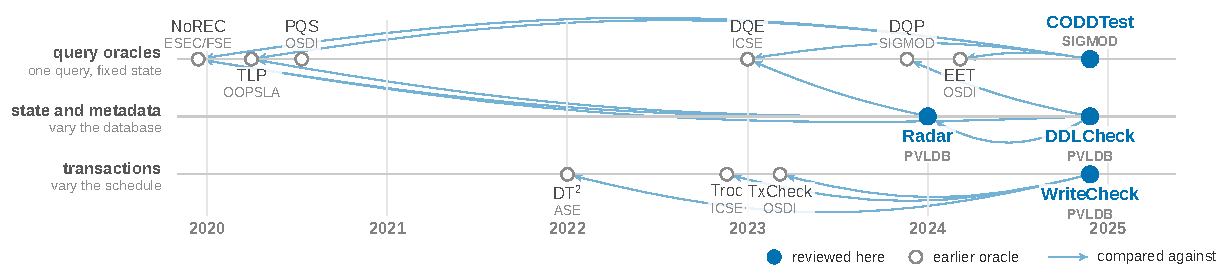
\includegraphics[width=\linewidth]{fig_lineage}
\caption{\textbf{Where the four papers sit in the oracle family, 2020--2025.} Lanes group oracles by what they vary; arcs point from each reviewed paper to the earlier tools it compares against in its evaluation. Venues from the papers' reference lists.}
\label{fig:lineage}
\end{figure*}

\begin{takeaway}
The four oracles are complements. Each sees a failure class the others cannot, and none sees a bug that corrupts both of its runs.
\end{takeaway}
